The projection of a satellite's orbit onto the Earth's surface is called its ground track. At a given instant, one can imagine a radial line drawn outward from the centre of the Earth to the satellite. The intersection between the Earth's spherical surface and this radial line is a point on the ground track.

The location of this point is specified by its geocentric latitude and longitude. The ground track is then essentially the figure traced by this point as the satellite moves around the Earth.

\textbf{Part I: Sun-Synchronous Orbits (25 points)}

It is particularly interesting to analyse the ground track of a so-called Sun-Synchronous orbit. This is a nearly polar orbit around a planet where the satellite passes over any given point on the planet's surface at the same mean local solar time. This property is especially interesting for satellite imaging, ensuring similar illumination conditions over different days.

The figure below shows the ground track of a satellite in a Sun-Synchronous orbit. Its inclination angle ($i$) - the angle between the satellite orbital plane and the Earth's equatorial plane - falls within the range $90^{\circ}<i<180^{\circ}$. The graph depicts five complete orbits of the satellite.

\begin{figure}[H]
    \centering
    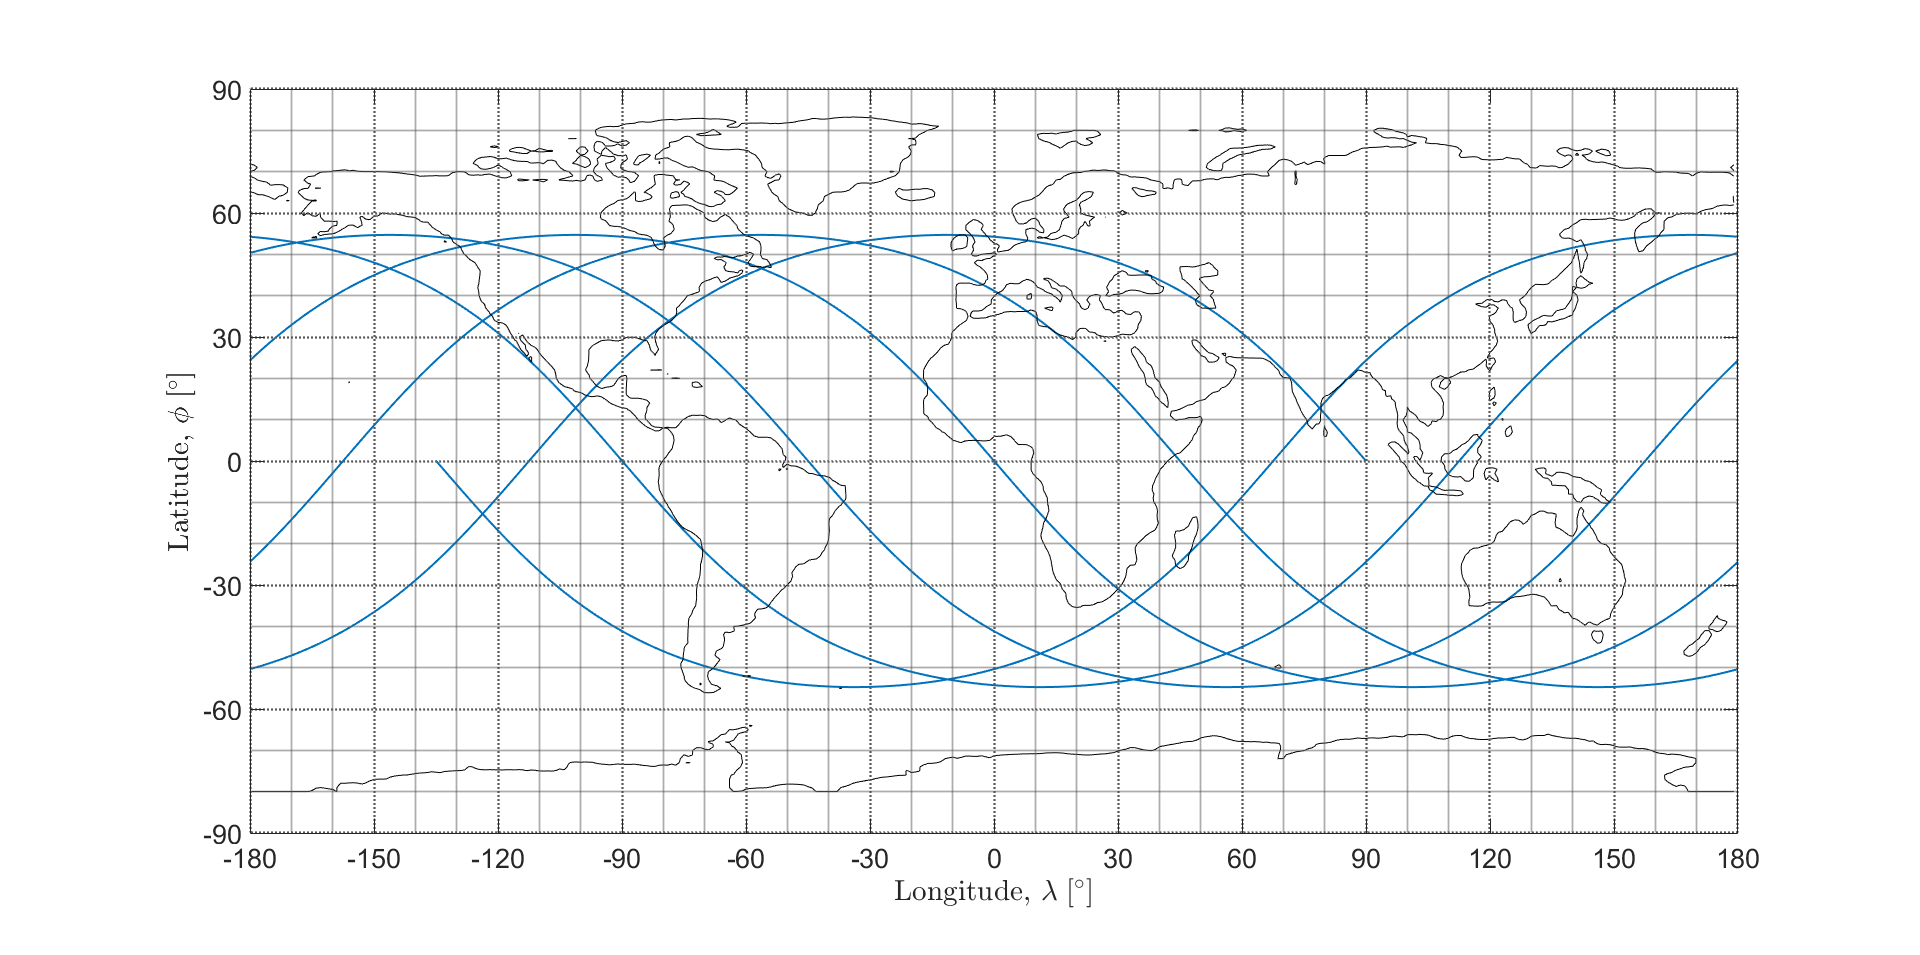
\includegraphics[width = 1\linewidth]{2024/Theory/Figures/2024_TH_Q11_F1.png}
    \caption{Ground Track for five orbits of the satellite}
\end{figure}

For the questions in Part I, assume that the Earth's orbit around the Sun is circular.
 
\begin{parts}
    \part[3]  Determine the nodal precession rate for the orbit in rad/s.
    
    \part[8] Based on the ground track shown in Figure 2, determine the inclination of the satellite's orbit (in degrees) and estimate its orbital period (in minutes). Consider that the orbital period of the satellite is shorter than one sidereal day.
    
    \part[2] Calculate the semi-major axis $a$ of the orbit in km.

    \part[1] Determine the number of orbits completed by the satellite until it returns to the same position on Earth.
    
    \part[11] {As seen in Figure 2, the ground track crosses the Brazilian city of Maceió $(\phi, \lambda) = (9.7^\circ S; 35.7^\circ W)$ and also Chorzów $(\phi, \lambda) = (50.3^\circ N; 19.0^\circ E)$, in Poland. Knowing that the ground track crosses Maceió at noon (local time), determine the local time that the satellite track crosses Chorzów. Hint: specifically for this task, you may neglect the effects of nodal precession}.

    \textbf{Part II: Tundra orbits (50 points)}
    
    A Tundra orbit is a type of geosynchronous elliptical orbit characterised by a high inclination. The apogee is positioned over a specific geographic region, allowing for prolonged visibility and coverage over that area. This orbit ensures that a satellite spends the majority of its orbital period over the northern - or southern hemisphere, making it particularly useful for communications and weather observation over high-latitude regions.
    
    The image below represents the ground track of a satellite in a Tundra orbit with an argument of perigee equal to $270^{\circ}$. The satellite orbits the Earth in the same direction as its rotation. For the following items, you can ignore the effects of the Earth's oblateness.
    
    \begin{figure}[H]
        \centering
        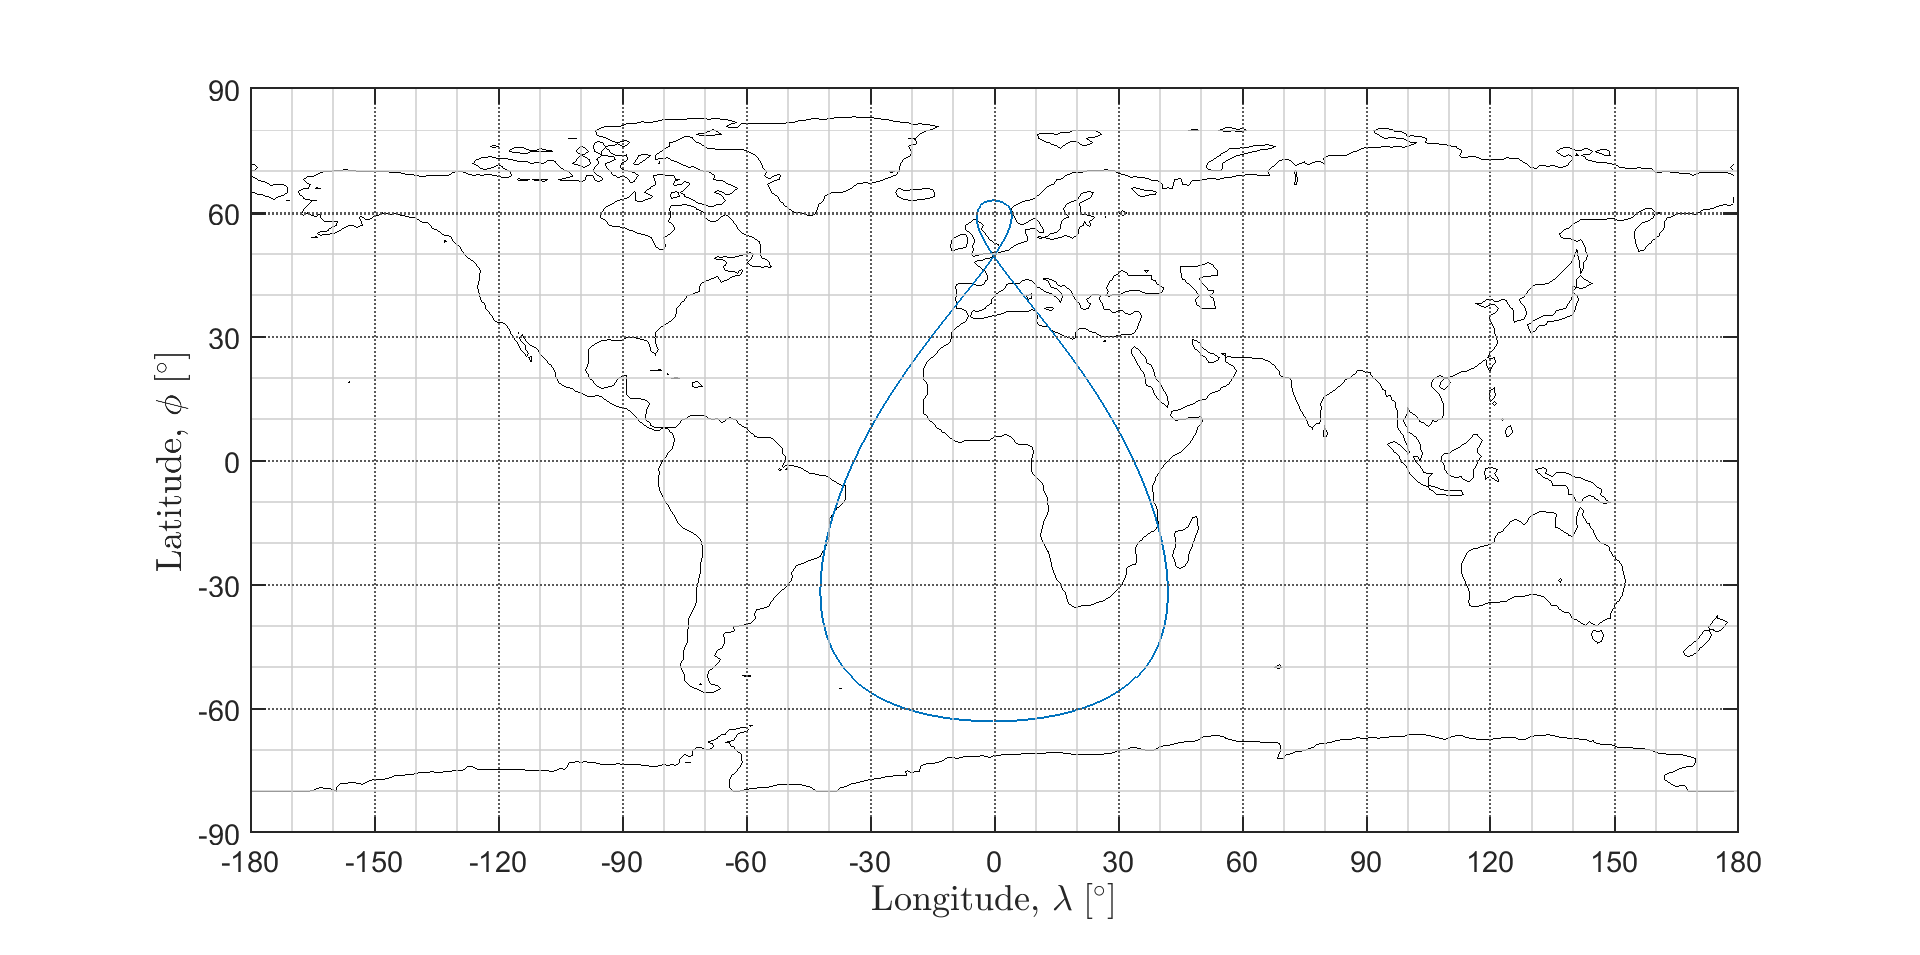
\includegraphics[width = 1\linewidth]{2024/Theory/Figures/2024_TH_Q11_F2.png}
        \caption{Tundra Orbit Ground Track for one orbital period}
    \end{figure}

    \part[4] Based on the graph above, give the inclination of the satellite's orbit \(i\) (in degrees), its orbital period \(T\) (in minutes), and its semi-major axis \(a\) (in km).

    \part[12] Show that the time a satellite spends in the northern hemisphere is given by
    
    $$
    T' = \left(\frac{1}{2} + \frac{\sin^{-1}(e)}{\pi} + \frac{e}{\pi}\cdot \sqrt{1 - e^2} \right) T
    $$
    
    where \(e\) is the eccentricity of the orbit and \(T\) is its orbital period.

    \part[10] Estimate numerically the eccentricity \( e \) of its orbit. You can consider that the eccentricity is so small that \(\sin(e) \approx e\) and \( e^2 \ll 1 \).

    \part[18] From the ground track, we can observe that the satellite exhibits retrograde motion in both its northern and southern hemisphere trajectories. Find the true anomaly (in degrees) of the satellite at the beginning and end of its retrograde motion in the southern hemisphere.

    \part[6] It is also noticeable that the ground track of a Tundra orbit has the shape of a figure-8, similar to an analemma, so that the satellite passes over the same point on Earth in a single orbit. Calculate the minimum eccentricity the orbit would need to have for this property to cease occurring. Use the same orbital inclination as the orbit in Figure 3.
\end{parts}